\documentclass{report}
\usepackage[english]{babel}
\usepackage{illcmolthesis}
\usepackage{microtype}
\usepackage{amsmath,amssymb}
\usepackage{amsthm}
\usepackage[round, authoryear]{natbib}
\usepackage[all]{xy}
\usepackage{array}
\usepackage{graphicx}
\usepackage{framed}
\usepackage{enumerate}
\usepackage{qtree}
\usepackage{mdframed}
\usepackage{tikz}
\usepackage{multirow}
\usepackage{pgfplots}
\pgfplotsset{compat = newest}
\usepackage{tikz-dependency}
\usepackage{xfrac}
\usepackage{algorithmic}
\usepackage{algorithm}
\usepackage{float}
\usepackage[OT2,T1]{fontenc}
\usepackage{hyperref}
\newcommand\textcyr[1]{{\fontencoding{OT2}\fontfamily{wncyr}\selectfont #1}}
\newcommand{\myparagraph}[1]{\paragraph{#1}\mbox{}\\}
\bibliographystyle{plainnat}
\renewcommand\topfraction{0.85}
\renewcommand\bottomfraction{0.85}
\renewcommand\textfraction{0.1}
\renewcommand\floatpagefraction{0.85}

%Define theorem style for definition and metric
\newtheoremstyle{break}  % follow `plain` defaults but change HEADSPACE.
  {\topsep}   % ABOVESPACE
  {15pt}   % BELOWSPACE
  {\itshape}  % BODYFONT
  {0pt}       % INDENT (empty value is the same as 0pt)
  {\bfseries} % HEADFONT
  {.}         % HEADPUNCT
  {\newline}  % HEADSPACE. `plain` default: {5pt plus 1pt minus 1pt}
  {}          % CUSTOM-HEAD-SPEC

\theoremstyle{break}
\newtheorem{metric}{Metric}
\newtheorem{notion}{Notion}
\newtheorem{definition}{Definition}
\def\citepos#1{\citeauthor{#1}'s (\citeyear{#1})}

%Define new float environment for tables that is boxed
\floatstyle{boxed}
\newfloat{tab}{tbp}{lop}
\floatname{tab}{Table}

\begin{document}
\chapter{Introduction}

%twee keer something?
Language and meaning play an important role in many aspects of our lives. When means of transportation and communication over larger distances became more publicly available, contact with other cultures became more prevalent and being able to understand how meanings are expressed in other languages than your mother tongue more important. Translation has something intriguing, as it seems to touch on something that is universal for all human beings, but is yet, even for human beings, a very nontrivial task. We would like to start this thesis with a famous quote of Warren Weaver, that we believe has, besides the author of current work, inspired many to pursue a career in machine translation:

\begin{quote}
\textit{``When I look at an article in Russian, I say: `This is really written in English, but it has been coded in some strange symbols. I will now proceed to decode.''} \citep{weaver1955translation}
\end{quote}

Evidently, automatic translation is not as easily solved as Weaver thought at the time. Over 60 years later, the state-of-the-art systems are still not able to produce translations of arbitrary pieces of text with a quality comparable to that of a human translation. This was not for the lack of trying: on Google Scholar one can found over 100,000 articles that contain the phrase ``Machine Translation'', of which almost 10,000 were published in the last two years.

Many different methods have been explored in these articles, one of which is called the transfer method. Contrary to more direct approaches that treat sentences as structureless sequences that can be translated into a sequence of words in another language more or less word for word, the transfer method aims to find structural representations for sentences in the source and target languages and finding a mapping between them. The translation process then consists of analysing the source sentence into a structure, mapping this structure to a target side structure, and generating a target sentence from this structure. A graphical representation of this process is shown in Figure \ref{fig:triangle}. The depicted pyramid shows that direct (word for word) translation can be seen as an extreme of the transfer method, in which the distance from the sentences to the intermediate representation is zero, and thus no analysis or generation takes place. On the other end of the spectrum we can find the case in which the intermediate representation is a universal one, independent of source and target language, and the mapping is the identity mapping. Such a universal intermediate representation of language is called an `interlingua'. 


\begin{figure}[!ht]
\centering
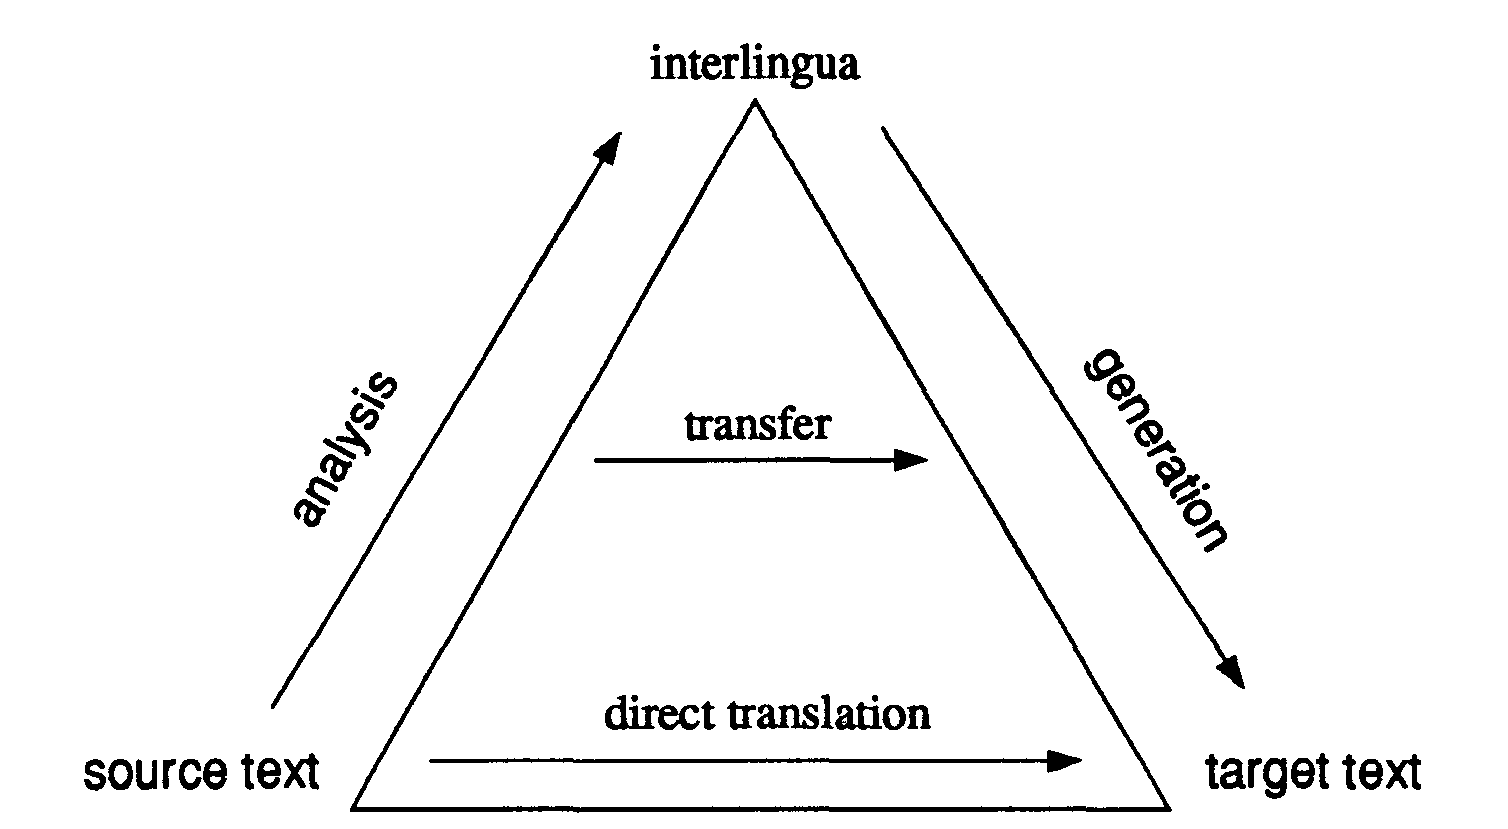
\includegraphics[scale=0.2]{translation_triangle.png}
\caption{Vauquois pyramid?}\label{fig:triangle}
\end{figure}

The pyramid also shows that transfer can be employed in many ways, varying the distance from intermediate representation to source and target language (analysis and generation, respectively). In this thesis, we consider the case in which the intermediate representations are interpreted as structural descriptions specifying how to derive the meaning of a sentence.\footnote{Theoretically, we believe this is the only interesting case of transfer, although transferring other types of information might be useful in practice} In other words, the underlying system generating these structures can be seen as a semantically motivated syntax of the language that specifies how the sentence was (compositionally) constructed with respect to its meaning. Hereby, it is important to notice that such a grammar is recursive, and the mapping between two of such grammars utilizing this fact can thus also be seen as compositional.

This type of transfer is theoretically interesting, as it addresses translation on a very fundamental level. However, although very many translation models have tried to incorporate transfer \citep[e.g.,][]{wu1997stochastic,chiang2005hierarchical}, and compositional methods of translation are theoretically well studied \citep[e.g.,][]{janssen1996compositionality}, it is not fully understood if translation from natural language to natural language can be treated in such a compositional fashion. In translation between other domains (logical languages, programming languages), compositional translation is almost trivially a sound approach, as the expressions of such languages are completely unambiguous and the compositional grammar according to which the meaning can be derived is known. Natural language has neither of these qualities, which does not only complicate the construction of a translation system, but also renders the existence of such a system uncertain.

In practice, the soundness of the approach can only be confirmed - by a machine successfully carrying out translation - and not refuted. Although many researchers have tried, the MT world is far from presenting such a machine. In theory, contrary to in practice, the soundness of the approach can only be refuted - by finding examples that can not be translated as such - and not confirmed. However, it turns out that theoretical examples of non-compositional translations (e.g., idiomatic translations), can often be dealt with elegantly in practice \citep{janssen1996compositionality}. Neither of these approaches thus seem to be promising with respect to determining whether it is possible to systematically construct structures for two languages and a mapping between them.

Nowadays, the availability of huge parallel corpora with texts that are manual translations of each other, together with techniques to align these corpora on the sentence and even word level, provide the means for a different approach. The alignments specify, on different levels of granularity, which units are each others translation and can therefore be interpreted as constraints on the structures possibly used in translation. In this thesis, we will empirically investigate how well these constraints, and the set of structures they give rise to, cohere with linguistic intuitions about language.

Other studies that empirically investigated the properties of translation data through alignments have focussed on the coverage of binary structures \citep[e.g.,][]{sogaard2009empirical1} and the extent to which conventional linguistic syntax oversteps the constraints set by alignment \citep[e.g.,][]{fox2002phrasal,hwa2002evaluating}. The latter studies show that monolingual syntax on its own is not suitable to deliver structures usable in translation, while the former studies provide formal information on the complexity of the reordering phenomena, but do not aim for a linguistic analysis of the multiple structures that can possibly be assigned to a sentence. 

In this thesis, we aim for a more general empirical approach that addresses both the formal and the linguistic side of the problem. We will do so by considering \textit{all} structures describing how a sentence could have been compositionally constructed that are in agreement with the alignment\footnote{As defined in \cite{simaan2013hats}}
(i.e., the set of structures that allow a compositional translation of the sentence), and aim to find one structure for each sentence, such that the resulting set of structures is consistent over the entire corpus, i.e., there is a systematicity in how the structures were derived. As we would like to link this systematicity to linguistic intuitions, we will consider the predicate-argument structures of the sentences as a starting point in this search. As they are closely related to the meaning of the sentence, we believe these structures have potential for being universal for language, and for largely agreeing with alignments. We will investigate how well these structures cohere with predicate argument structures, and analyse the causes in which they deviate from each other.

The contributions of this paper are thus twofold. Firstly, we will investigate the preservation of predicate argument structures across different language pairs. As this yields an empirical view on the universality of such structures, this is interesting for the field of linguistics in general. Secondly, we will aim to devise a method to enrich translation corpora with recursive translation structures based on linguistic intuitions, and shed a light on the difficulties that arise in doing so. The latter is interesting for the field of machine translation, most clearly because it broadens the perspective on the sufficiency of the transfer method, to which it is directly related. Furthermore, a structurally consistent treebank for a parallel corpus might serve as a starting point for a new MT model, and the open source implementation produced for this thesis could prove useful for developing one.


\section*{Thesis Outline}

\bibliography{thesisDH}
\end{document}